\section{Interactive physically based Fluid and Erosion Simulation}
The behaviour of water massively influences the look and features of a terrain. Depending on the timespawn, amount of water, ground composition and many more factors, hydraulic erosion creates a variety of different, but distinctive ground deformations, such as ripples, ridges, meanders, riverruns and valleys. 
This paper \cite{Neidhold:2005:IPB:2381356.2381361} presents an approach capable of creating such deformations in short amount of time, making it suitable for interactive visualization. The model represents terrain and water surfaces using heightfield, which is sampled onto a regular grid. A shallow water model is used to update the water surfaces and the fluid velocity field. 

\subsection{Water simulation}
This paper uses a simplified Navier-Stokes equation to simulate the water flow. The approach discards 3D-features like mutiple water layers, vertical vortices and waves. this makes the equation less physically correct, but much faster to compute. The appraoch is based on a system of first order differential equations. This system describes the movement of material, in this case the amount of water at each cell, depending on velocity $\vec{v}$ and acceleration $\vec{a}$. Since this approach is dealing with complex erosion, the system uses am multidimensional material vector storing additional parameters like dissolved sediment.
$$\dot{\vec{v}} = \vec{a} -K_A \cdot \vec{v}=\frac{\vec{F}}{m} - K_A\cdot \vec{v}$$
$$K_A$$ describes the friction between the fluid and the terrain and can be manipulated for test purposes. 

\begin{figure}
	\centering
	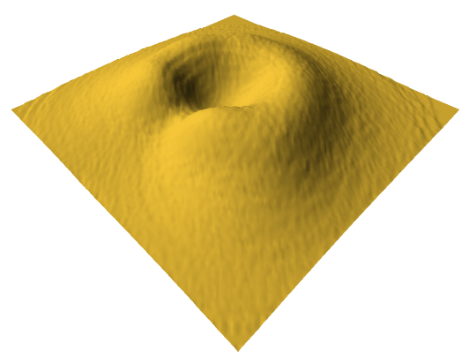
\includegraphics[width=\linewidth]{NWD05/hydraulic_errosion_a}
	\caption{Original model}
	\label{fig:calc_acceleration}
\end{figure}

\begin{figure}
	\centering
	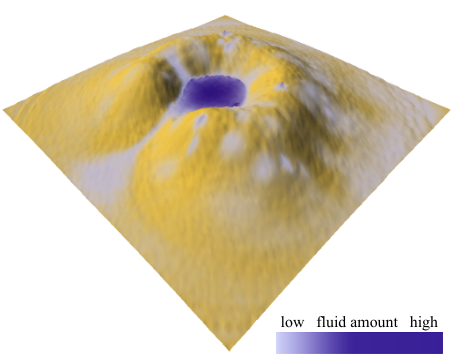
\includegraphics[width=\linewidth]{NWD05/hydraulic_errosion_b}
	\caption{Fluid simulation}
	\label{fig:calc_acceleration}
\end{figure}

A vector field assumes that the particles movement is constant. In a common Newtonian Physic System objects are accerlated by the gravity. The direction of acceleration is the direction of the biggest tile angle $\alpha$ of the underlying height field. Therefore the acceleration force can be computed from the sinus of $\alpha$ times the gravitational constant g. The angle $\alpha$ is determined by the gradient $\nabla I(x,y)$ of the height field. 

At this point he acceleration direction is only defined in x and y direction. The acceleration vector $\vec{M}$ can be computed using the gradient $\nabla I(x,y)$: 
$$\vec{M} = (- \frac{\Delta I}{\Delta x}, - \frac{\Delta I}{\Delta y}, - \frac{\Delta I^2}{\Delta x^2}, - \frac{\Delta I^2}{\Delta y^2})^T$$
The acceleration vector can now be computed as follow: 
$$\vec{a}= \frac{|\vec{M}_z|}{|\vec{M}|} \cdot g \cdot \frac{\vec{M}}{|\vec{M}|}$$

$\vec{M}_z$ describes the acceleration direction direction along the z axis.

\begin{figure}[htb]
	\centering
	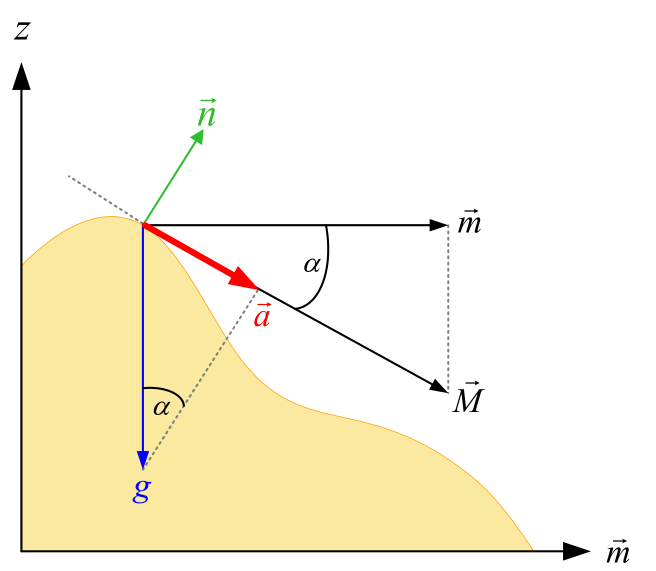
\includegraphics[width=.8\linewidth]{NWD05/acceleration}
	\caption{Calculation of acceleration.}
	\label{fig:calc_acceleration}
\end{figure}

\subsection{Hydraulic erosion function}
When water flows, soil, stones and other materials are dislocated and transported to lower regions. Whenever a part of material is moved to another grid cell by the simulation a hydraulic erosion function is used. It determines the amount of disolved and deposited parts of material. The function uses the amount of transported fluit $\Delta F$ and the amount of sediment dissolved in this fuild $\Delta S$ as input. The function determines whether sediment can be deposited to or dissolved from the underlying cell. The function uses three major constants. 
\begin{itemize}
\item A \textbf{sediment capacity constant} $K_C$ determines how much of the underlying material can be dissolved per unit of water at a velocity of one. 
\item \textbf{The deposition constant} $K_D$ controls the rate at wich soil is deposited at the target grid cell. 
\item The \textbf{dissolving constant} $K_S$ controls the dissolving rate of the underlying terrain into the fluid per simulation step.
\end{itemize}

The sediment capacity $c_S$ speficies the maximum amount of sediment that can be transported by the fluid $\Delta F$. $\Delta t$ scales the equation corectly at time steps unequal to one.  
$$ c_S = \frac{K_C}{\Delta t} \cdot \Delta F  \cdot |\vec{v}|
$$
If the amount of dissolved sediment $\Delta S$ exceeds the sediment capacity $c_S$, deposition is happening, otherwhise the fluids capacity is not yet used fully, therefore more material is dissolved into the liquid. 

If $\Delta S > c_S$ deposit: 
$$
H = H + \frac{K_D}{\Delta t} \cdot ( \Delta S - c_S )
$$
$$
S = S + \Delta S - \frac{K_D}{\Delta t} \cdot (\Delta S - c_S)
$$
If $\Delta S <= c_S$ dissolve: 
$$
H = H + \frac{K_S}{\Delta t} \cdot ( \Delta S - c_S )
$$
$$
S = S + \Delta S - \frac{K_S}{\Delta t} \cdot (\Delta S - c_S)
$$

Both cases modify the height H of the terrain at the given cell. Depositing increases the height and decreases the sediment dissolved in the fluid, whilst dissolving dcreases the height H and increases the sediment amount in the fluid. The material constants $K_D$, resp. $K_S$ additionally scale the equation for erosion of different materials. 

\begin{figure}
	\centering
	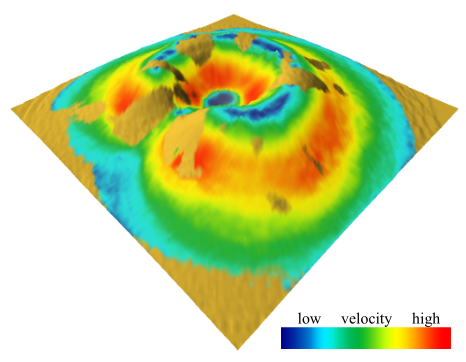
\includegraphics[width=\linewidth]{NWD05/hydraulic_errosion_c}
	\caption{Color-coded fluid velocity}
	\label{fig:calc_acceleration}
\end{figure}

\begin{figure}
	\centering
	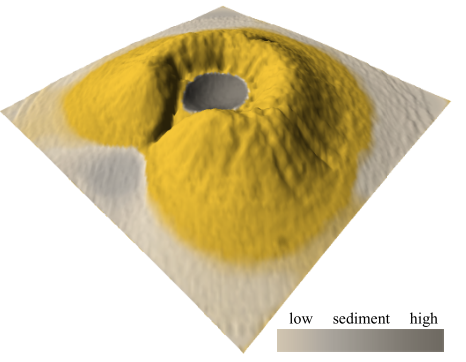
\includegraphics[width=\linewidth]{NWD05/hydraulic_errosion_d}
	\caption{Eroded terrain after 300 simulations steps with color-coded depositing}
	\label{fig:calc_acceleration}
\end{figure}